\subsubsection{Añadir}\label{addPreguntaAsesor}

  \paragraph{}Para añadir un nuevo elemento al sistema, es necesario pulsar el
  icono \textit{Añadir nuevo}. Se puede ver una captura de pantalla de este
  icono en la figura \ref{capturaAddElemento}.

  \paragraph{}Al pulsar en el icono, se enlazará con el formulario de creación
  del nuevo elemento. Este formulario se puede ver en la imagen
  \ref{capturaAddPreguntaAsesor}.

  \begin{figure}[!ht]
    \begin{center}
      \fbox{
      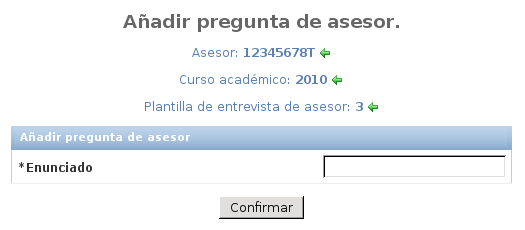
\includegraphics[scale=0.55]{4.Funcionamiento_Aplicacion/4.3.Gestion/4.3.1.Administrador_Principal/4.3.1.21.PreguntaAsesor/add_pregunta_asesor.png}
      }
      \caption{Captura de pantalla del formulario para la creación de \textit{Pregunta de asesor}.}
      \label{capturaAddPreguntaAsesor}
    \end{center}
  \end{figure}

  \paragraph{}Una vez rellenado el formulario, se pulsará el botón
  \textit{Confirmar}, el cual se puede ver en la figura
  \ref{capturaBotonConfirmar}. Si el formulario rellenado es válido, y no tiene
  errores, se creará el nuevo elemento en el sistema. En caso de contener
  información no válida, un mensaje de error aparecerá indicando los campos
  del formulario que no han pasado la validación, los cuales habrá que modificar
  para introducir correctamente el elemento en el sistema.